\chapter{Discussão de resultados}

\par Neste capítulo serão apresentados e discutidos os resultados obtidos pela pesquisa e implementação 
do sistema de otimização do processo de fabricação de calças. Tal discussão será realizada em forma de
casos de teste, buscando demonstrar o comportamento do algoritmo genético de diferentes formas.

\par Desde o princípio, quando começamos a discutir sobre o tema do nosso trabalho de conclusão de curso, tínhamos em mente
desenvolver algo relacionado à inteligência artificial, por ser um assunto de bastante relevância na área de desenvolvimento
de software. Dentro deste campo então, realizando algumas buscas na internet, encontramos o assunto de algoritmos genéticos.
Coincidentemente no primeiro semestre deste ano, tivemos aulas de sistemas especialistas a qual o assunto foi abordado o que facilitou bastante o aprendizado. 

\par Assim, como sugestão do professor Roberto Rocha, decidimos então desenvolver uma aplicação para otimizar um processo de
distribuição de atividades entre costureiras para um microempresário da cidade de Cachoeira de Minas - MG do ramo de costura e 
constatamos que um sistema Web seria mais cômodo de ser utilizado por não precisar de nenhuma instalação e o usuário poder
acessar o programa de qualquer lugar desde que estivesse conectado à internet, neste sentido, como já estávamos familiarizados
com JSF e Primefaces decidimos adotá-los como tecnologias para o desenvolvimento em plataforma Web, além disso usamos um 
\textit{plug-in} denominado \texttt{JBoss Tool} o qual foi de grande utilidade para gerar as classes modelo a partir do 
banco de dados.

\par Inicialmente tomamos como base o caso do microempresário citado acima, todavia logo após iniciarmos o trabalho, o mesmo fez uma 
reestruturação de processos em sua empresa. Desta forma, sua maneira de trabalhar deixou de ser um cenário o qual algoritmos genéticos
pudessem ser aplicados, desta forma, decidimos fechar um escopo para que o trabalho pudesse continuar, conforme descrito na seção 
reuniões do quadro metodológico. Com o escopo definido, o foco passou a ser na definição da estrutura dos elementos do algoritmo genético. 

\par Como já explanado no quadro teórico, segundo \citeonline{livro_ags_ricardo_linden}, a estrutura do algoritmo genético é composta
por populações que são formadas por indivíduos que por sua vez são formados por cromossomos.
Cada indivíduo representa uma solução e cada cromossomo do indivíduo representa uma de suas características. 
Assim então é gerado uma população inicial de indivíduos e, a partir desta, um processo de cruzamento 
e mutação é iniciado a fim de que possa ser gerados novos indivíduos que representem soluções ainda melhores 
que seus antecessores.

\par Uma das maiores dificuldades nesta etapa, foi definir como os indivíduos e cromossomos seriam estruturados. Assim em uma discussão com o professor Artur Barbosa, decidimos que o total de peças deveriam ser divididos em lotes e que cada cromossomo deveria ter uma costureira 
e a quantidade de lote a ser confeccionado por esta, assim o indivíduo teria um conjunto de cromossomos que representaria quais costureiras 
e o quanto elas iriam trabalhar naquele processo, representando uma solução para a distribuição.

\par Com base nesta definição, um dos papeis desempenhados pelo algoritmo, seria a distribuição aleatória do trabalho. Neste
sentido, nos deparamos com uma outra dificuldade que foi a de definir a população inicial de indivíduos, ou seja, 
como os lotes de peças seriam distribuídos para cada cromossomo. Inicialmente pensamos em distribuir porcentagens para cada costureira
e posteriormente fazer um cálculo de normalização, conforme explica a sessão Distribuição das atividades do quadro metodológico porém,
constatamos que o cálculo não era preciso e que, ao cruzar dois indivíduos, os indivíduos filhos, após o cálculo de normalização, ficavam
completamente diferente de seus progenitores fugindo assim da ideia de algoritmos genéticos. Definimos então distribuir as atividades já 
nível de lote o que resolveu a questão. 

\par Um dos maiores desafios do trabalho foi a definição da função de avaliação, pois, uma vez que existe uma estrutura de nós contendo
as atividades e o cálculo do tempo de cada atividade depende de nós predecessores, a maior parte da função foi pensada para ser 
desenvolvida de forma recursiva o que dificultou o \texttt{debug}. 

\par Para a construção do algoritmo genético, foi utilizado uma base desenvolvida pelo professor Artur Barbosa durante as aulas de sistemas especialistas, que define uma série de regras a ser seguida durante o desenvolvimento tal base é explicada com mais detalhes no quadro metodológico. Tal base foi de grande ajuda pois, além de definir tais regras de desenvolvimento a base já implementava os métodos de 
seleção e cruzamento, neste sentido só tivemos que realizar algumas adaptações nestes para que pudessem se adequar à nossa lógica.

\par Após ter o escopo definido e a modelagem do algoritmo genético realizada, dividimos o desenvolvimento entre os autores
e mantivemos reuniões periódicas para acertar detalhes do desenvolvimento.

\par Após todas as etapas descritas acima, obtivemos como resultado a aplicação capaz de distribuir atividades de forma a se obter o 
menor custo e o menor tempo de produção, alcançando assim nossos objetivos específicos. 

\par Com a aplicação finalizada, foram realizados então casos de testes a fim de colocar em prova a eficiência da ferramenta para se 
buscar melhores soluções nas distribuição de tarefas, conforme mostra as sessões abaixo.


\section{Teste com somente uma atividade}
\par Este teste foi realizado com apenas uma atividade, neste caso não está sendo considerado que as costureiras devem ir 
até a fábrica para retirar os tecidos com o Marcelo. Para este teste foi cadastrado então um processo, criando-se apenas uma atividade para 
este, conforme mostra a Figura abaixo:

\begin{figure}[h!]
	\centerline{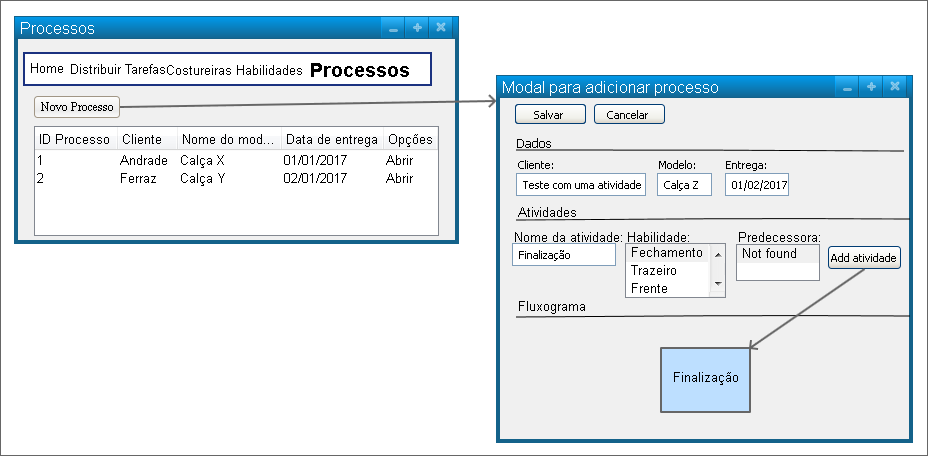
\includegraphics[scale=0.4]{./imagens/test_case_1.png}}
	\caption[Caso de teste]
	{Caso de teste com uma atividade \textbf{Fonte:} Desenvolvido pelos autores}
	\label{fig:exemplo1}
\end{figure}

\par Para a atividade de finalização, atribuída ao processo na Figura acima, foram cadastradas 5 costureiras e seus respectivos
tempos para fazer tal atividade, conforme mostra a Figura abaixo:

\begin{figure}[h!]
	\centerline{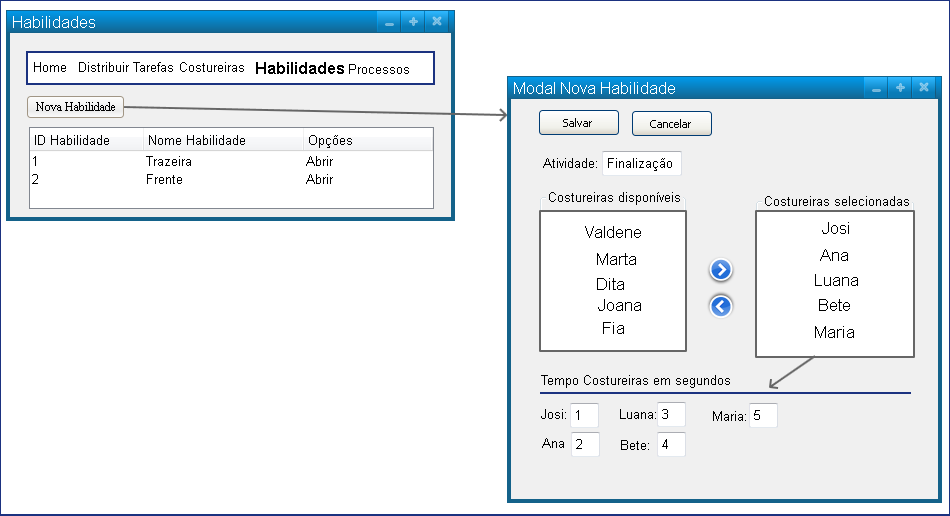
\includegraphics[scale=0.4]{./imagens/test_case_1_habilidades.png}}
	\caption[Caso de teste Habilidade]
	{Cadastro da habilidade e associação das costureiras \textbf{Fonte:} Desenvolvido pelos autores}
	\label{fig:exemplo1}
\end{figure}

\par Feito isso foi iniciado então o processo de distribuição das atividades, através do menu Distribuição de Tarefas.
O algoritmo foi configurado para ter 1000 gerações e 80 indivíduos em cada população, além disso a taxa de indivíduos
estrangeiros e de mutação foram de 0,5\% e 0,05\% respectivamente, conforme mostra a figura abaixo. 

\begin{figure}[h!]
	\centerline{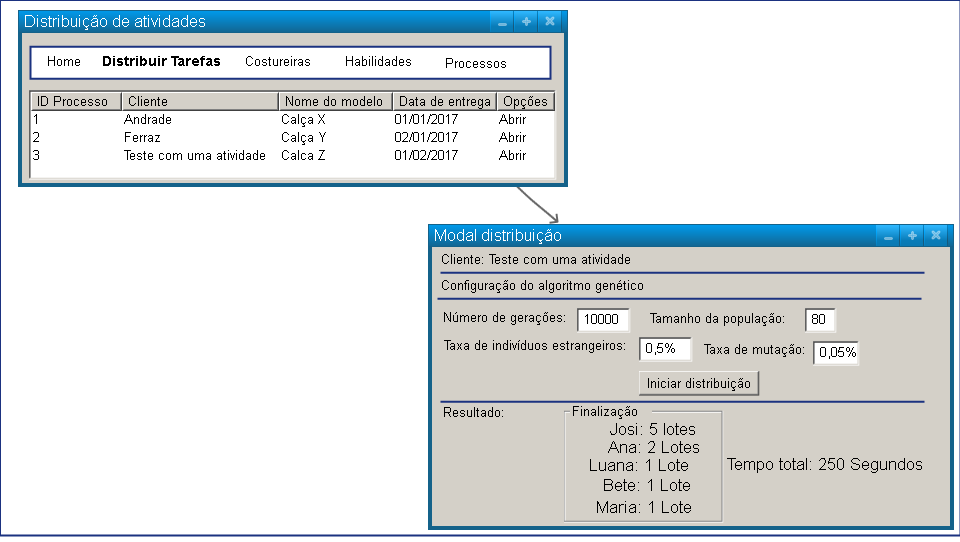
\includegraphics[scale=0.4]{./imagens/test_case1_distribuicao.png}}
	\caption[Caso de teste Habilidade]
	{Distribuição das atividades \textbf{Fonte:} Desenvolvido pelos autores}
	\label{fig:exemplo1}
\end{figure}

\par Após clicar no botão "Iniciar Distribuição", o algoritmo distribuiu os lotes para as costureiras da finalização,
conforme mostra a Figura X. O tempo total encontrado foi de 250 segundos. Este é o tempo da costureira que demorou mais
tempo para produzir seus lotes. Na Figura 27, pode-se ver o tempo gasto por cada costureira, de acordo com seu tempo de
produção para cada peça.


\begin{figure}[h!]
	\centerline{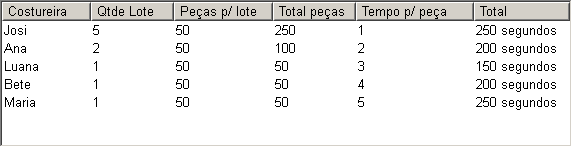
\includegraphics[scale=0.6]{./imagens/test_case1_resultado.png}}
	\caption[Caso de teste Habilidade]
	{Resultado da distribuição \textbf{Fonte:} Desenvolvido pelos autores}
	\label{fig:exemplo1}
\end{figure}

\par Baseando-se na Figura 27, pode-se observar que o algoritmo distribui o máximo de peças possível para a Josi, porque
ela tem o menor tempo. Nota-se que 5 é o máximo de lotes que a Josi pode receber porque se ela recebesse mais um, seu 
tempo total passaria a ser 300 segundos, assim o tempo total não seria de 250 segundos. Assim o algoritmo distribuiu as 
atividades as outras costureiras de forma uniforme, porém, de forma inteligente, definiu menos lotes para aquelas que 
gastam mais tempo para se produzir, ou seja, encontrou a melhor forma de distribuir as tarefas para este caso provando assim
sua eficiência.

\section{Teste considerando o tempo de transporte}
\par Este teste foi realizado com duas atividades em que as costureiras estão em suas casas. Neste caso deve-se considerar
o tempo de transporte entre as costureiras da atividade Frente e a fábrica do Marcelo para a retirada dos materiais e o tempo 
entre tais costureiras e a costureira responsável pela finalização, conforme mostra a Figura 31.


\begin{figure}[h!]
	\centerline{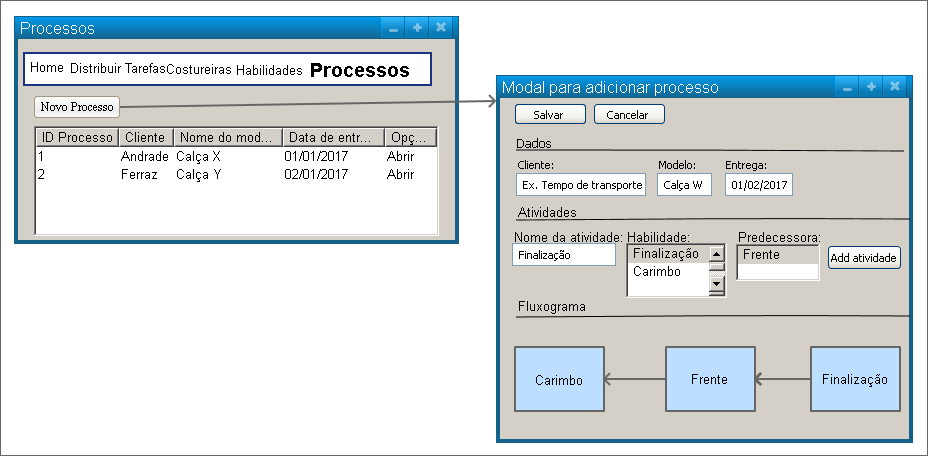
\includegraphics[scale=0.3]{./imagens/test_case_2.png}}
	\caption[Caso de teste tempo]
	{Caso de teste com tempo de distribuição \textbf{Fonte:} Desenvolvido pelos autores}
	\label{fig:exemplo1}
\end{figure}


\par Neste teste foi considerado apenas o tempo de transporte, logo o tempo de confecção por peça das costureiras da parte 
da Frente possuem o mesmo valor, conforme mostra a Figura 32.


\begin{figure}[h!]
	\centerline{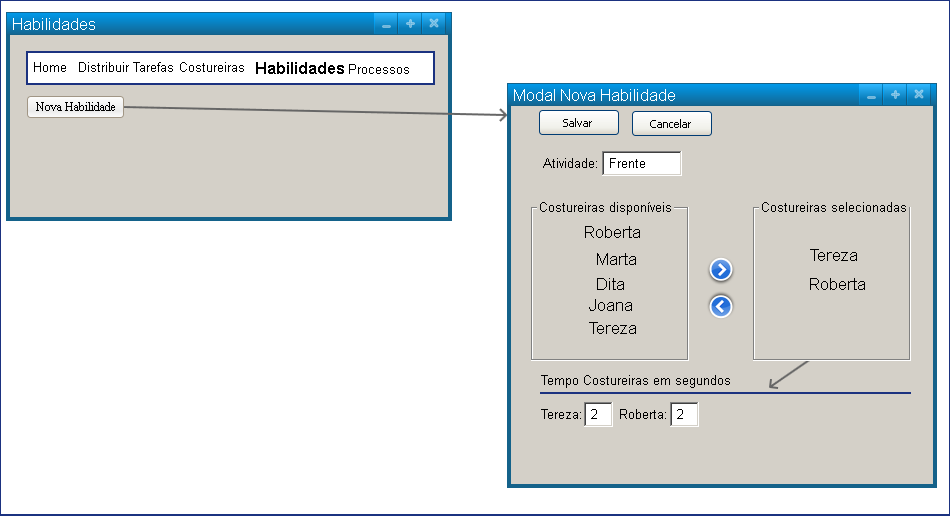
\includegraphics[scale=0.3]{./imagens/test_case_2_habilidades.png}}
	\caption[Caso de teste tempo]
	{Caso de teste com tempo de distribuição \textbf{Fonte:} Desenvolvido pelos autores}
	\label{fig:exemplo1}
\end{figure}

\newpage

\par Além disso foi necessário cadastrar um valor X e Y para cada costureira que representa sua localização conforme 
mostra a Figura 33.


\begin{figure}[h!]
	\centerline{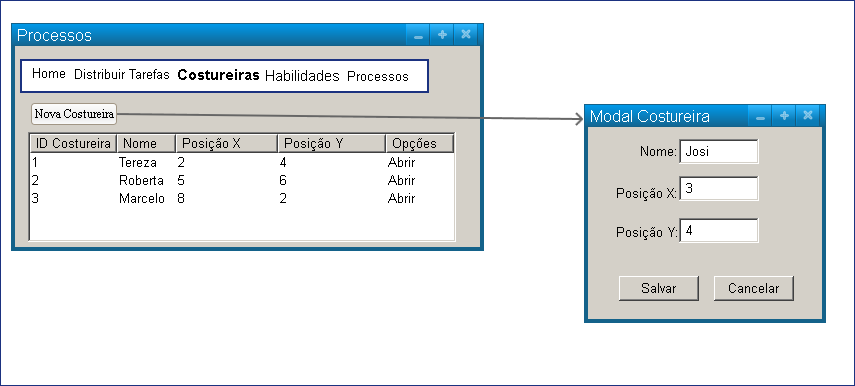
\includegraphics[scale=0.3]{./imagens/test_case_2_costureiras.png}}
	\caption[Caso de teste tempo Costureira]
	{Cadastro de costureiras \textbf{Fonte:} Desenvolvido pelos autores}
	\label{fig:exemplo1}
\end{figure}

\par \par Feito isso foi iniciado então o processo de distribuição das atividades, através do menu Distribuição de Tarefas.
O algoritmo foi configurado para ter 1000 gerações e 80 indivíduos em cada população, além disso a taxa de indivíduos
estrangeiros e de mutação foram de 0,5\% e 0,05\% respectivamente, conforme mostra a figura abaixo. 

\begin{figure}[h!]
	\centerline{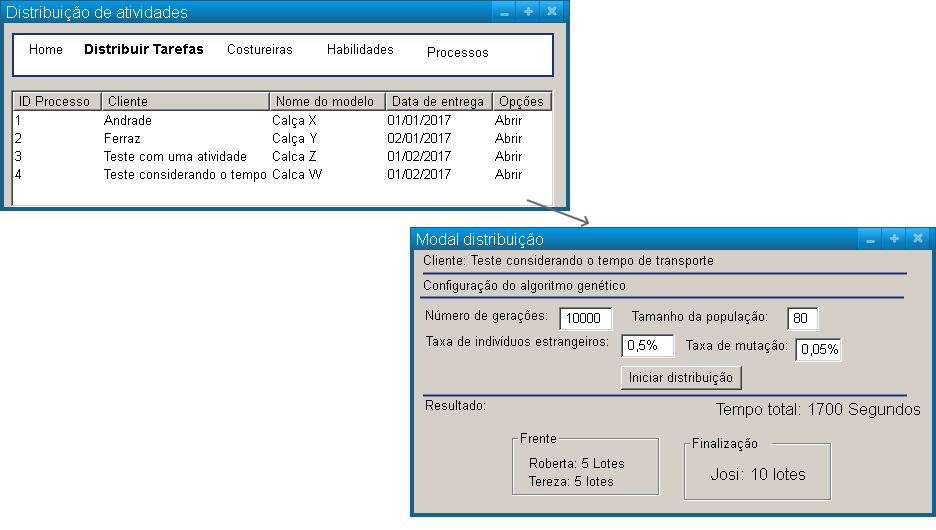
\includegraphics[scale=0.3]{./imagens/test_case2_distribuicao.png}}
	\caption[Caso de teste tempo Costureira]
	{Distribuição das atividades \textbf{Fonte:} Desenvolvido pelos autores}
	\label{fig:exemplo1}
\end{figure}

\par Após clicar no botão "Iniciar Distribuição", o algoritmo distribuiu os lotes para as costureiras das atividades
 finalização e frente e o tempo total encontrado foi de 1700 segundos, conforme mostra a Figura 34. Neste caso o algoritmo 
 distribuiu 5 peças para cada costureira da parte da frente, logo, como a atividade de finalização possui somente uma costureira,
 a Roberta e a Tereza irão passar 5 peças cada uma para a Josi que faz a finalização. Conforme descrito no quadro metodológico, 
 o cálculo da distância entre as costureiras é realizado através da fórmula euclidiana multiplicando-se o resultado por 100.
 A Figura 35 mostra as distâncias entre as costureiras calculadas através desta fórmula com suas posições X e Y.
  
  \newpage
  
  \begin{figure}[h!]
  	\centerline{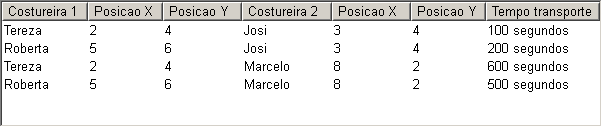
\includegraphics[scale=0.7]{./imagens/test_case_2_tempo_distribuicao.png}}
  	\caption[Caso de teste tempo Costureira]
  	{Distribuição do tempo  \textbf{Fonte:} Desenvolvido pelos autores}
  	\label{fig:exemplo1}
  \end{figure}
 
\par Considerando que as costureiras Roberta e Tereza gastam o mesmo tempo para fazer a frente e que o tempo de transporte 
entre a Tereza e a Josi é menor (100 a menos que entre a Roberta e a Josi), o algoritmo deveria distribuir mais peças a Tereza,
porém os materiais devem ser pegos na casa do Marcelo e, neste caso, o tempo de transporte entre a Tereza e o Marcelo é 100 
a mais que o tempo de transporte entre a Roberta e o Marcelo, logo o algoritmo entendeu que o tempo se igualou e definiu
o mesmo número de peças para cada costureira.

\par Existem outros resultados a serem documentados incluindo a questão de custo, porém até a entrega da discussão dos resultados
os mesmos não estavam elaborados.
